\chapter{Standards, Standard Englishes,\\and what to teach}\label{sec:standards}\label{ch:standards}

\epigraph{standards stand guard
at every gate we pass through,
measuring the distance 
between what we say\\\phantom{~}\hfill
and what they hear}{}

In \hyperref[ch:categories]{the next chapter}, I'll return to describing the lexical categories, but here, we should spend some time considering a few issues that are all connected to perceptions of what is right and wrong when it comes to English. This chapter should help you think about the concepts of standards\is{standard|(}, Standard English(es)\is{Standard English|(}, grammaticality\is{grammaticality|(}, and normativity\is{normativity|(}~-- all of which are crucial for English language teachers to understand.

Why are these concepts important? Well, as teachers, we're often asked to be the arbiters of what's ``correct'' in English. But as you'll see, it's not always as straightforward as it might seem. What's standard? What's grammatical? And perhaps most importantly, what should we actually teach?

We'll start by unpacking the concept of ``standard'' and how it applies to language. Then we'll explore the notion of Standard English~-- or rather, Standard Englishes~-- and why this distinction matters. We'll dive deep into grammaticality\is{grammaticality!questioning of|(}, examining what makes something grammatical\is{grammatical!vs meaningful|(} or ungrammatical\is{ungrammaticality}, and why our intuitions\is{intuition!about grammaticality|(} about this can sometimes be misleading. Finally, we'll consider the normative aspects of language and how they impact our decisions as teachers.

By the end of this chapter, you should have a more nuanced understanding of these concepts and be better equipped to navigate the complex landscape of English language teaching. So, let's begin by considering what we mean when we say something is ``standard''.

For most people, \textit{standard} has positive connotations\is{standard!positive connotations of}. Consider the words that we use together with \textit{standard}, pairs like \textit{gold standard} and \textit{quality standard},  or \textit{standard of living} and \textit{standard of care}. If you have high standards or exceed them, that's a good thing. We set educational standards, environmental standards, and technology standards\is{technology standard}\is{technology standard|(}, all of which are supposed to make our education, environment, and technology better.

Standards, in short, are things we aspire to and \textit{Standard English} (note the capital~\textit{S}) may sound like something to aim for. You might think it's equivalent to ``good'' English, grammatical\is{grammatical!vs Standard English|(} English, or literary English. But it's not that simple, not that clear, not that straightforward to define or aim for.

You're likely old enough to know what VHS is. What you may be too young to know, though, is what Betamax is. Back in the early 1980s, they were \href{https://en.wikipedia.org/wiki/Videotape_format_war}{competing video tape standards}. By most criteria, Betamax was a higher quality product. It had a better picture and better sound. Nevertheless, it died so long ago that you may never have heard of it, and VHS became the standard for video cassette tape and players (at least while people still used VCRs).

Standard doesn't mean good, and good doesn't mean standard.

There are a lot of different rail gauges (Fig. \ref{fig:rail}), but standard rail gauge\is{standard!rail gauge analogy} is 1.435 m wide. That's what they're using for a new light rail line in Mississauga, where I live. Toronto gauge, the one traditionally used by the Toronto Transit Commission (TTC), one city to the east, though, is 1.495 m wide. To be sure, each size has benefits and drawbacks, but the main benefit of standard rail gauge is that it is standard. It is the most commonly used, and so if you want new rail cars, or even used rail cars, it's much cheaper and faster to get them if you use standard gauge. That's why Mississauga chose it, despite meaning that rolling stock will not be able to interchange directly with Toronto's system. The choice was not about quality or superiority; it was about cost and availability. 

Standard English\is{Standard English!not inherently superior|(} is not the ``best'' form of English. Standard English is not inherently superior to other dialects\is{dialect!and Standard English|(}. Standard English is simply the most widely accepted, the most institutionalized, the most common ground for diverse communication\is{communication!as function of language}.

In linguistics, the term \textsc{standard} often serves more as a sociopolitical marker\is{Standard English!as a sociopolitical marker} than a qualitative one. It is a product of historical, cultural, and often colonial forces that have elevated one dialect~-- usually that of a socially or economically dominant group~-- over others. 

So, when we talk about Standard English, what we're really discussing is a set of conventions that have been codified and are taught in schools, used in official documents, and expected in formal settings. It is not a measure of intelligence, morality, or worth; it is simply what is most commonly and broadly expected and accepted. And it's what most folks have in mind when they say they want to learn to speak English. The word \textit{standard} in Standard English is less about quality and more about ubiquity and institutional backing. It's the VHS, not necessarily the Betamax, of the English language.

\begin{figure}
\centering
\includegraphics[width=0.7\textwidth]{figures/Track_gauge.svg.png}
\caption{Track gauge}
\label{fig:rail}
\end{figure}

Standards \href{https://www.wired.com/2002/01/standards-2/}{underpin our modern world}, but standards are often arbitrary\is{standard!arbitrary nature of|(}. A4 paper is the standard in most of the world, so A4 is better there. US Letter is the standard in North America, so US Letter is better there. Neither is inherently superior; their superiority comes from being standard.

Standard English follows this pattern. It's not inherently better; it's better because it's standard. Many Englishes could be standard, if only they were.

But there are two important differences between technology standards\is{technology standard!vs language standards|(} and language standards\is{language standard!vs technology standards|(}. First, a technology standard is stipulated. Somebody planned it out and promulgated it. Language isn't like that. Second, if you don't follow a technology standard, your technology often won't work. A TTC streetcar, for instance, simply will not run on standard gauge rails. It's useless as a means of transportation. Similarly, a VHS cassette simply will not play on a Betamax player. In contrast, much of the time~-- perhaps most of the time~-- non-standard English is a perfectly workable means of communication\is{communication!and non-standard English}, even with speakers of Standard English. There are dialects and varieties that you or I cannot understand~-- or cannot understand easily~-- but there are so many more that we can. If communication is the main function of language, then, why do we have Standard English?

One answer is that another function of language is to regulate group membership\is{group membership!and dialect|(}. In other words, language helps us to identify people who are like us, who belong to our group. Young people often create a sense of identity and belonging within their peer groups by developing, innovating, and using slang. For example, \textit{fire} as an adjective meaning `excellent' gained significant traction among teens in the early 2000s. Those who used it then used it as a way of saying, ``I'm part of this group that knows this new meaning of \textit{fire}, and because I use it with you, it means I think you are too.'' Of course, adults were rarely, if ever, part of the group, and they rarely, if ever, used \textit{fire} that way.

Or consider clothing. Jeans are standard at most colleges and universities in Canada. Some people wear suits or dresses, which are more formal but still standard ways of dressing. Arriving topless to class might be perfectly functional if the classroom is warm, but it's not standard, and people will react to such a choice of outfit with surprise and discomfort. A snowsuit is also non-standard, as is a sari, a chef's uniform, or a man's kilt. Some people on campus will react positively and some negatively. Many will suppress any outward reaction, but everyone will recognize that these ways of dressing are non-standard.

That's kind of the way it is with non-Standard Englishes. If you use one of them, people will notice. Standard English is a social standard, and it has social implications. Usually those are negative for those who don't speak Standard English, and as language teachers, we should recognize that our students' goals are often as social as they are instrumental. They want to learn English so that they can function in society, but they want to learn Standard English so that they will be a part of it\is{standard!arbitrary nature of|)}\is{technology standard|)}.


\section{Standard English(es)}\label{sec:standard}

George Eliot presents the following conversation in her novel \textit{Middlemarch}.

\begin{quote}
    ``All choice of words is slang. It marks a class.''

    ``There is correct English: that is not slang.''

    ``I beg your pardon: correct English is the slang of prigs who write history and essays. And the strongest slang of all is the slang of poets.''
\end{quote}


Eliot knew the difference between ``correct English'' and Standard English. But many people don't. Unfortunately, there is no brief definition\is{Standard English!definition (lack of brief)} of Standard English that I can use to clarify it (more difficulties with definitions). In fact, one goal of this book is to outline a partial definition of the syntax, vocabulary, and phonology of Standard English. But I can at least make a few remarks about its dominant status.

To some degree any dialect of English is a standard among some group, but most are not called ``Standard English''. If you try to sell a Standard gauge train to the TTC for its subway, you will not make a sale; Standard gauge is not the standard used in Toronto.

If you grew up speaking \href{https://en.wikipedia.org/wiki/Indigenous_English_in_Canada}{First-Nations English}\is{dialect!First-Nations English}, then First-Nations English is likely the standard in your home community; anyone who goes to your community and speaks Standard English will mark themselves as outsiders and will be treated as such, for good or ill.

And to be clear, there isn't a single Standard English. There's Standard Canadian English\is{Standard English!Canadian}, Standard British English\is{Standard English!British}, Standard Singapore English\is{Standard English!Singapore}, etc. For the most part, these are almost indistinguishable, at least when written down, but there are small differences; the unique aspects of any of the varieties will often jump out at speakers of another. Still, they are all recognized as Standard English, or more recently as Standard Englishes.

But let me reiterate that this is not because Standard English is better, more formal, or even most common (though it is the most common is particular communities).\footnote{For more about what it isn't, see \citet{trudgill99}.} \textit{Standard} is not synonymous with \textit{grammatical} or \textit{correct}. Nor does it imply truth, logic, beauty, purity or clarity. It is not how English ``ought'' to be spoken. It is just a cluster of dialects\is{Standard English!as a cluster of dialects}, albeit a powerful one, and a norm that is enforced by the dominant social group of English speakers. In much of the world, that means educated speakers of English from Britain and the former British colonies where the Indigenous peoples were largely displaced (e.g., Canada), but not those where the Indigenous peoples were not (e.g., Bangladesh)\is{Standard English!not inherently superior|)}\is{dialect!and Standard English|)}.

\begin{tcolorbox}[title=What's a shibboleth\is{shibboleth|(}?, colback=white] \label{sec:shibboleth}
    There is a story about the gate-keeping function\is{shibboleth!gate-keeping function} of dialects in Judges, the 7\textsuperscript{th}
    book of the Hebrew bible, which goes like this.
    
    \begin{quote}
        Jephthah then called together the men of Gilead and fought against Ephraim. The Gileadites struck them down because the Ephraimites had said, ``You Gileadites are renegades from Ephraim and Manasseh.'' The Gileadites captured the fords of the Jordan leading to Ephraim, and whenever a survivor of Ephraim said, ``Let me cross over,'' the men of Gilead asked him, ``Are you an Ephraimite?'' If he replied, ``No,'' they said, ``All right, say \textit{Shibboleth}.'' If he said, ``Sibboleth,'' because he could not pronounce the word correctly, they seized him and killed him at the fords of the Jordan. Forty-two thousand Ephraimites were killed at that time. --Judges 12:4 (NIV)
    \end{quote}
    
    From this story, we get the English word \textit{shibboleth}\is{shibboleth!origin of term}, a manner of speech distinguishing a particular group of people, often used as a means of identification or a test of belonging. The term \textit{shibboleth} now signifies any type of linguistic or cultural indicator that separates ``insiders'' from ``outsiders.'' In the modern usage, a shibboleth might not be a matter of life and death, but it can still significantly influence how we perceive and interact with others.
    
\end{tcolorbox}

\section{Questioning grammaticality} \label{sec:questioning-grammaticality}

When I was first hired as an English teacher, it wasn't because of my qualifications. I had none. Nor was it because of my experience. As I said, it was my first teaching job. Nevertheless, I arrived in Japan in November of 1992, and within two weeks, I had been hired. I assume this was I because I am a ``native speaker'' of Standard English. Being white probably helped, too.

As someone who grew up speaking Standard English, I was obviously a competent user of the language, but I had little explicit grammatical knowledge. Most schools in Canada teach essentially nothing at all about English grammar. That was true in the 1970s and 80s, when I was in school, and it remains true today. I was lucky in that I was among the first wave of \href{https://en.wikipedia.org/wiki/French_immersion#Canada}{French immersion} students, and so I knew something about (French) grammar at least. But this was only the tiniest help to me when I tried to address my students' questions.

``Why do you use the present continuous here, but the present simple there?'' ``When do we need \textit{the}?'' ``Why do we ask \textit{who \uline{does} she know} but not usually \textit{who \uline{does} know her}?'' To all of these questions, I could say little more than, ``it sounds right.'' I had strong intuitions\is{intuition!about grammaticality} about what was grammatical and what was not, but I had no way of conveying those intuitions to my students in any systematic and generalizable way. I'd never even thought about what it means for something to be grammatical.

At this point, you~-- yes, you~-- already have much more explicit knowledge of English grammar than I did. In fact, you probably have more explicit knowledge about English grammar than the average college professor. If a student asked you about the determiners in \textit{I had coffee and a piece of toast for breakfast}, you could tell them that \textit{coffee} is an non-count noun, so it doesn't require a determiner, but, as a singular count noun, \textit{piece} can't go without (see Section \ref{sec:count}). You know something about English grammar. So you're way ahead of where I was when I started out.

But you still probably haven't thought about what it means for something to be grammatical. This is what I'd like to explore here. (A fuller treatment is given in Chapter \ref{ch:grammaticality}.)

\begin{tcolorbox}[title=The fallacy of monosemy\is{fallacy of monosemy|(}, colback=white] \label{sec:fallacy-of-monosemy}\is{monosemy}
    Before we dive in, though, just a few words about the fallacy of monosemy. If a word is monosemic, it has a single (\textit{mono--}) meaning (\textit{\uline{sem}antics)}. This is the idea at play when a child asks, ``can I go to the toilet,'' and the teacher responds cruelly, ``I don't know, \textit{can} you?'' The teacher acts as though \textit{can} really has only one meaning, `ability', when in fact \href{https://www.ldoceonline.com/dictionary/can}{\textit{can}} has multiple meanings. In Chapter 1, I mentioned technical meanings and everyday meanings. When somebody says, ``technically the word means $x$,'' they could simply be saying that there is a technical sense of the word, but more often they're falling into the fallacy of monosemy.
\end{tcolorbox}\label{sec:monosemy}

We don't need to pretend that \textit{grammatical} has only one true meaning, but nor does it mean just anything. How do we establish the meaning of \textit{grammatical}? As the comic in Figure \ref{fig:comic} explains, what a word means depends on what we mean when we use it.

So, spend some time thinking about what \textit{grammatical} and \textit{ungrammatical} mean to you. Recall cases in which you've used them. What were you referring to? If not, consider creating some examples for each. Either way, try to think of commonalities that might generalize to other examples, especially if some borderline cases occur to you.

\begin{figure}
\centering
\includegraphics[width=0.95\textwidth]{figures/hotdogSandwich1.png}
\end{figure}

\begin{figure}
\centering
\includegraphics[width=0.90\textwidth]{figures/hotdogSandwich2.png}
\caption{Is a Hotdog a Sandwich? A Definitive Study, from \textit{\href{https://existentialcomics.com/}{Existential Comics}} by Corey Mohler.}
\label{fig:comic}
\end{figure}

\textit{The concise Oxford dictionary of linguistics} \citep{Matthews2003} defines \textit{grammatical} like this.


\begin{enumerate}[noitemsep]
    \item Having to do with grammar [\dots].
    \item Specifically of sentences, etc. which conform to the rules of a given language: e.g. \textit{I like tea }is grammatical in English, while \textit{I tea like} is ungrammatical. Hence grammaticality\is{grammaticality!definition} or grammaticalness is variously a property either assigned to sentences by a specific grammar, or of sentences judged to be acceptable to speakers who hypothetically `know' its grammar.
\end{enumerate}

Are we reduced to Wittgenstein's notion that language is mere use? That whatever we say is grammatical? That our speech defines our grammar? Well, yes, but that's of no help to you or your students, so I would like to consider some examples.

Let's start with an easy one.


\ea[]{\textit{Me key there happy mine the}.}
\label{ex:key}
\z


I hope you agree that (\ref{ex:key}) seems unequivocally ungrammatical\is{ungrammaticality!example of|(}. But why? No, really, why? If you feel that it is ungrammatical, what can you point to to support that intuition? If somebody claimed that this is actually grammatical, what counter-arguments could we make?

Well, we could start with \textit{key} and say that, as a singular countable noun, it needs a determiner and it doesn't seem to have one (see Section \ref{sec:count}). An NP like \textit{my} could function as a determiner, but \textit{me} doesn't function that way, at least not in Standard English, though perhaps this is the \textit{me} of a different dialect wherein \textit{me} can mean ``my''. You could look at \textit{key} and ask yourself whether it's a noun or a verb. If it's a noun, then there is no verb, and if this is supposed to be a clause, it needs a VP as its head (see Section \ref{sec:verbs}). So, let's assume \textit{key} is a verb. That makes \textit{me} the subject, but we would expect \textit{I} here, not \textit{me}. And if \textit{key} is a verb, then you expect to key something. Unfortunately, \textit{there} and \textit{happy} aren't somethings that can be keyed. You could say, \textit{please key mine}, but \textit{mine} seems too detached from \textit{key} for that to work. And \textit{the} is just left at the end there, in a position where it never occurs.

I could go on, but perhaps it's simpler than that. Maybe (\ref{ex:key}) is ungrammatical because it doesn't make sense. Could it be that grammatical language always makes sense? Could it be that something that makes sense is grammatical? (These are not the same claims.) As critical thinkers, we need to try to disprove our ideas. We could do this by creating a grammatical utterance that makes no sense and comparing it to an ungrammatical utterance. Fortunately, the hugely influential linguist Noam Chomsky has done that for us already with the famous (at least in linguistics) examples in (\ref{ex:greenIdeas}).

\ea
    \ea[]{\textit{Colorless green ideas sleep furiously.}}
    \label{ex:greenIdeas1}
    \ex[*]{\textit{Furiously ideas sleep green colorless.}}
    \label{ex:greenIdeas2}
    \z
    \label{ex:greenIdeas}
\z

\begin{figure}
    \centering
    \includegraphics[width=3in]{figures/green-ideas.jpg}
    \caption{Colorless green ideas sleep furiously, from \citep{parkvall2008limits}.}
    \label{fig:greenIdeas}
\end{figure}

\textcite[16]{Chomsky2002-ko} claims that (\ref{ex:greenIdeas1}) is grammatical and that (\ref{ex:greenIdeas2}) is ungrammatical, which matches my intuition (and yours too, I expect). It seems, you don't have to make sense to be grammatical.


But Chomsky also claims that neither the sentences nor their subparts would occur in a corpus of English, and they would be ``equally `remote' from English [\dots] in any statistical model of English''. He wants to say that frequency has nothing to do with it. Here, I think he errs. Fernando \textcite{Pereira2000} has shown that (\ref{ex:greenIdeas1}) is actually much more statistically likely than (\ref{ex:greenIdeas2}). And the success of large language models like ChatGPT shows that language truly is built on statistical regularities\is{grammaticality!and statistics} \citep{Kallini2024}.

Next, we'll consider the converse, that all meaningful language is grammatical. Before we do, try to think of something that is ungrammatical but has a clear meaning.

Now consider (\ref{ex:JeanPaul}).

\ea[]{\textit{Jean Paul, very very good.}}
\label{ex:JeanPaul}
\z

This example was heard by my friend, Geoff Pullum, in an interview on NPR. As he explains in \href{http://itre.cis.upenn.edu/~myl/languagelog/archives/003830.html}{this blog post}, the speaker was Turkish. Her meaning, in its context, is clearly that Pope John Paul was a very, very good pope or person. But for this to be grammatical in English, we need a clause, with a subject and a head. That head should be a VP, which means we need a verb, presumably \textit{be}, but another verb that licenses predicative complements, such as \textit{seem} or \textit{become}, would also be possible.

It seems, then, that something can be grammatical but not meaningful\is{grammatical!vs meaningful} and meaningful but not grammatical\is{meaning!and grammaticality|(}. So meaning is neither a necessary nor sufficient condition for grammaticality.\is{necessary and sufficient conditions}

So, here's another thought: perhaps we just go by the rules in grammar books\is{grammaticality!and rule books}.

\ea
    \ea[]{\textit{He was a beautiful young man, a beautiful beautiful boy.}}\label{ex:beautifulboy} 
    \ex[*]{\textit{The boy was beautiful beautiful.}}\label{ex:beautifulboy2}
    \z
\z

As you can tell by the star, I think (\ref{ex:beautifulboy}) is grammatical, but not (\ref{ex:beautifulboy2}). I assume you agree. The rule that explains this appears in \textit{CGEL} (p. 561) and was first noted, I believe, by \textcite{Watt1968}. But it is not widely known, and I assume that you've never encountered it before. I also assume that the grammaticality of (\ref{ex:beautifulboy}) and (\ref{ex:beautifulboy2}) didn't change in 1968, when Watt wrote his article about it, or in 2002, when \textit{CGEL} was published. Given that, I guess we can set aside the idea that rules in grammar books dictate what is grammatical. Many rules are not mentioned in grammar books. In fact, many languages exist without any linguist having written a grammar for them at all. We wouldn't want to say that anything goes in those languages, just because no books have been written about them.

Now consider (\ref{ex:whmovement}).

\ea[*]{\textit{What movies do you have friends who acted in?}}
\label{ex:whmovement}
\z

Probably, you'll agree that this is a very strange sentence, almost like an optical illusion, feeling grammatical and ungrammatical at the same time. The reason is thought to be the result of something called \href{https://en.wikipedia.org/wiki/Wh-movement#Extraction_islands}{island constraints}\is{island constraint}, a kind of rule or limitation that many linguists think might apply to all languages, though there is some debate about this. This could be the result of some processing constraint\is{processing limitations!and grammaticality|(} in our brains, or it could be something about how information can be structured. Fortunately, if this is true, then you'll never have to explain it to your students, because nobody would naively try to use a sentence like this.

So it seems that our processing ability may help us decide what is grammatical and what is not. With this in mind, consider which image in Figure \ref{fig:suitcases} is described by (\ref{ex:suitcase}).

\ea[]{\textit{After the trip, my suitcase sat unpacked on the floor for days.}}
\label{ex:suitcase}
\z

\begin{figure}
    \centering
    \includegraphics[width=2in]{figures/full_suitcase.png}
    \includegraphics[width=2in]{figures/empty_suitcase.png}
    \caption{Which suitcase is unpacked?}
    \label{fig:suitcases}
\end{figure}

Many people say this is the first suitcase~-- the one on the left with the clothes in it~-- but that is incorrect. The first suitcase is packed. You put clothes in when you pack a suitcase. The second one has been unpacked; all the clothes have been removed.

Why would anybody get this wrong? The people who have thought about this question often feel that there's something tricky in the negation, the \textit{un--} at the beginning of \textit{unpacked}. After all, if you replaced it with \textit{packed}, the meaning would be perfectly clear. So, is there some kind of glitch in the way we process language that messes with our comprehension sometimes? Maybe we can't rely on instinct to judge what is grammatical at all. In fact, this is exactly what (\ref{ex:horse}) suggests.

\ea[]{\textit{The horse raced past the barn fell.}}
\label{ex:horse}
\z

I expect that (\ref{ex:horse}), another sentence famous in linguistics, from \citet{bever1971}, seems ungrammatical to you, but you may have noticed that there is no star. What if we change \textit{raced} to \textit{ridden}? Now it is clearly grammatical (if it's not yet clear, it means `the horse that was raced past the barn fell'). The problem you had with (\ref{ex:horse}) was that you interpreted \textit{raced} as the past-tense form (like \textit{rode}) rather than the past-participle form (like \textit{ridden}). Again, maybe our instinct isn't 100\% reliable. Sometimes, we need to think things through carefully, step-by-step.

When it comes to (\ref{ex:30years}), it seems to me that this is perfectly grammatical (compare: \textit{I have 30 dollars}). In fact, this is how ages are discussed in many languages. But even though it's grammatical, it's still the wrong way to say \textit{I'm 30 years old}, at least in English. So even being grammatical isn't the same as being acceptable\is{grammatical!vs acceptable}.
\ea[\textsuperscript{?}]{\textit{I have 30 years.}}
\label{ex:30years}
\z

North American speakers of English generally judge (\ref{ex:weekend}) to be ungrammatical, but it is the normal way to express \textit{I'll see you on the weekend} in British English.

\ea[\textsuperscript{\%}]{\textit{I'll see you at the weekend.}}
\label{ex:weekend}
\z

This is one of the small differences among Standard Englishes\is{Standard English!regional differences} I mentioned in Section \ref{sec:standard}, and the `!' marks it as differing between varieties of Standard English. The reason for this difference is not a grammatical one, bur rather that we are operating under different cultural assumptions about the relevant metaphor\is{metaphor!for weekend (platform vs point)} for weekends: it has been claimed that North Americans see a weekend as a platform or stage on which events play out, while the British see it as a point at the end of the week.\footnote{See Section \ref{sec:preposition-meanings} for more about metaphors and prepositions.}

\ea[\textsuperscript{!}]{\textit{I ain't no quitter.}}
\label{ex:quitter}
\z

Like (\ref{ex:weekend}), (\ref{ex:quitter}) is not ``wrong'' but rather an example of a dialectal difference. It may not be grammatical in Standard English, but it is in other varieties.

\ea[]{\textit{Me and Mia are taking the bus.}}
\label{ex:bus}
\z

In contrast (\ref{ex:bus}) is fully grammatical in all dialects, but it belongs to an informal register\is{style restrictions (formal, informal, etc.)!and register}. The more formal version would use \textit{Mia and I}. This is a shibboleth\is{shibboleth!example of} for some people.

Finally, try to fix (\ref{ex:bad-and}), which I find ungrammatical.
\ea[*]{\textit{Jim and me's teacher was Geoff.}}
\label{ex:bad-and}
\z

There's no good solution here. If we change it to \textit{Jim and my}, then it's like `my teacher and Jim', which is not what I mean, and a similar problem applies to \textit{me and Jim's}. But *\textit{Jim and my's} sounds just as ungrammatical as *\textit{Jim and me's}. Could it be that we need to be ungrammatical sometimes in order to express certain simple concepts? I think that might be the case\is{ungrammaticality!example of|)}\is{fallacy of monosemy|)}\is{intuition!about grammaticality|)}\is{meaning!and grammaticality|)}\is{processing limitations!and grammaticality|)}\is{grammaticality!questioning of|)}\is{grammatical!vs meaningful|)}.

\subsection{Summary}

Generally, things that are grammatical are meaningful and vice versa, but being meaningful is neither necessary nor sufficient for grammaticality. Many of the rules are described in grammar books, but many aren't (and often the description in grammars are just wrong). Expert users of English can generally rely on our intuition to know what is grammatical, but our intuition can be fooled\is{intuition!fallibility of|(}. Sometimes, an explanation helps us to see something we didn't before. Some grammatical things are just not what we'd say, and some things just can't be said grammatically. So, what makes grammatical grammatical?

\section{A model of grammaticality} \label{sec:gramm-model}

Okay, so we've seen that grammaticality isn't as straightforward as we might have thought. But that doesn't mean we can't come up with a useful way of thinking about it. Here's a model\is{grammaticality!model of|(} that might help.

At its core, grammaticality is about form--meaning pairings\is{form--meaning!pairing|(} that work for a particular group of speakers in a particular situation. It's not universal. Figure \ref{fig:speaker_groups} shows just a few of those groups. To see what I mean, consider that a teen saying \textit{mommy sock} to mean `that's your sock, mom' feels very ungrammatical (and very odd). The same utterance by an infant doesn't evoke either of those feelings, though, because it's a good form--meaning pairing that works for a particular group of speakers in a particular situation.

Or consider the following conversation from \citet[179]{nishimura1995}. The text in italics is Japanese\il{Japanese}, and the translation is in single quotes.

\begin{quote}
    B.C. \textit{ni iku toki} (`When I went to B.C.'), \textit{hikōki de yomoo to omotte kara} (`thinking I would read it on the plane'), I bought it, eh? So, it's not finished yet. (Laughs) And it's hard, 'cause me\textit{-nanka} (`a person like me'), \textit{mō} (`really'), \textit{hon-nanka yomu to} (`when I read a book'), cover-to-cover \textit{yomanakattara} (`unless I read it cover-to-cover'), if I stop \textit{dokka de }(`at some point'), I forget the story.
\end{quote}

This kind of code-switching\is{code-switching!and grammaticality}\is{code-switching!example of} is perfectly grammatical for any English--Japanese bilingual, but much of it seems ungrammatical for other English speakers.

\begin{figure}[ht] \label{fig:speaker-groups}
\centering
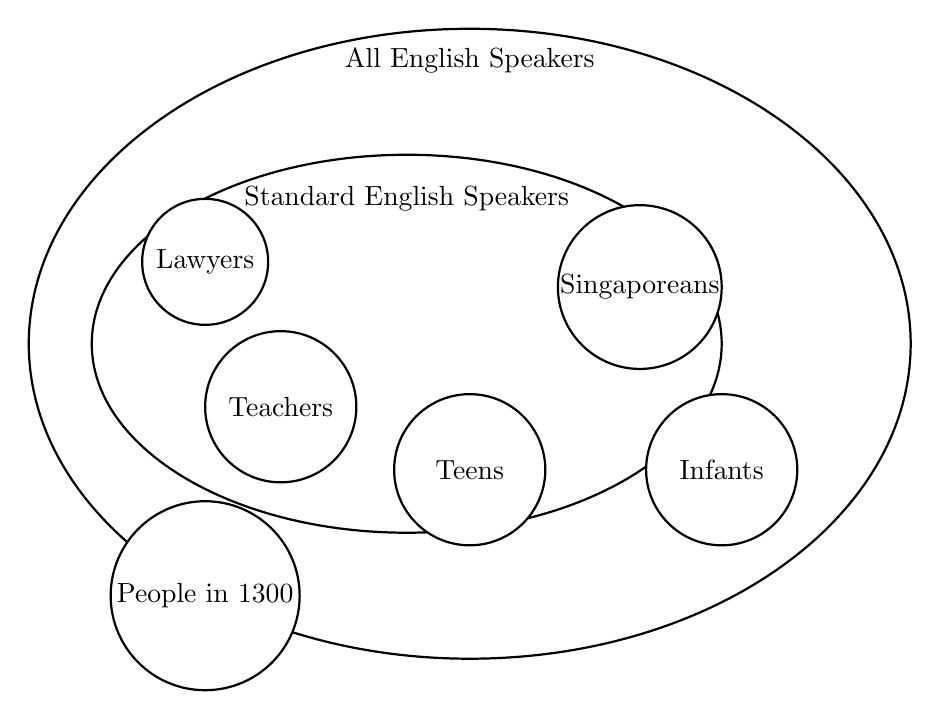
\begin{tikzpicture}[scale=0.8]
    % Main ellipse for all English speakers
    \draw[fill=white, thick] (0,0) ellipse (7cm and 5cm);
    \node at (0,4.5) {All English Speakers};
    
    % Ellipse for Standard English speakers
    \draw[fill=white, thick] (-1,0) ellipse (5cm and 3cm);
    \node at (-1,2.3) {Standard English Speakers};
    
    % Smaller ellipses for different groups
    \draw[fill=white, thick] (-3,-1) circle (1.2cm);
    \node at (-3,-1) {Teachers};
    
    \draw[fill=white, thick] (0,-2) circle (1.2cm);
    \node at (0,-2) {Teens};
    
    \draw[fill=white, thick] (2.7,0.9) circle (1.3cm);
    \node at (2.7,0.9) {Singaporeans};
    
    \draw[fill=white, thick] (4,-2) circle (1.2cm);
    \node at (4,-2) {Infants};
    
    \draw[fill=white, thick] (-4.2,1.3) circle (1cm);
    \node at (-4.2,1.3) {Lawyers};
    
    \draw[fill=white, thick] (-4.2,-4) circle (1.5cm);
    \node at (-4.2,-4) {People in 1300};
    
\end{tikzpicture}
\caption{Relationship among groups of English speakers (not to scale).}
\label{fig:speaker_groups}
\end{figure}


When it comes to the meaning\is{meaning!context-dependent|(}, there can often be layers and layers, any of which need to match the construction used to convey them. \textit{Try it and you'll regret it} has literal meaning\is{meaning!literal vs implied}: an instruction to try something followed by a predication that the experience will lead to regret. In everyday speech, though, it has a conditional meaning: `if you try it, you'll regret it'. On top of those, it also may carry an implied threat: `if you do that, I will punish you'. Here, the literal meaning of imperative \textit{try it} is turned on its head and comes to mean `don't try it'.

Sometimes old constructions pair with new meanings. That's how we ended up with the \textit{going to} future-time idiom: it began literally meaning going somewhere to do something (e.g., \textit{Why am I going there? I'm going to shop.}), but the fact that the activity could only happen after some period of travel time provided the opportunity for it to take on a futurate meaning. Other times grammatical constructions becomes less grammatical or falls out of use. Take the way we make questions and negatives in English, for instance. Shakespeare would have asked \textit{know you not?} instead of \textit{don't you know?}, and obviously, that's not how you and I say it.



So when do we say something's ungrammatical? A few situations come to mind. First, when the form doesn't pair with or even suggest any meaning at all, like \textit{Can the have running?} Second, when there's a mismatch between what you mean and what people expect you to mean. \textit{I have 12 years} is a perfectly good way of replying to the question \textit{How long do you have until retirement?} but it's ungrammatical\is{ungrammaticality!conditions for|(} in response to the question \textit{How old are you?}


Third, when you've got contradictory form--meaning pairs\is{form--meaning!pairing!contradictory} in the same utterance. \textit{I have two job} tells us both that that number of jobs is plural and that it's singular. And finally, when there's a strongly preferred alternative form, and there's no good reason not to use it.

Take a common phrase like \textit{It's very good}. Most English speakers would call this grammatical. Say \textit{It very good} instead, and you'll still get your meaning across~-- after all, ungrammatical doesn't mean meaningless. But listeners might pause, wondering why you skipped the verb. Maybe you're quoting something? Referencing a meme? Without a clear reason for the unusual form, they're likely to judge it ungrammatical.

These judgments aren't always reliable guides. Our brains sometimes flag perfectly grammatical sentences as wrong just because they're tricky to process. Other times, we breeze right past actually ungrammatical phrases without noticing, especially in casual conversation when we're focused on meaning rather than form.

This model frames grammaticality not as following rules from grammar books but as being about using form-meaning pairs that work for your linguistic community in a given context\is{context!and grammaticality|(}. Grammar isn't hardwired into our brains~-- despite what many linguists since the 1950s have claimed.\footnote{For example, we don't have innate principles and parameters the way \citet{chomsky1981lectures} claimed.} Language is fluid, shaped by its speakers. What counts as grammatical shifts across time, space, and social groups.

Most learners aim their speech at the Standard English-speaking world. Not everyone needs or wants to match these standards exactly. Many just want to communicate effectively~-- maybe to do business in a country like Vietnam. When students pursue Standard English, we guide them toward that goal. Fortunately, unlike rigid technical standards, language standards\is{language standard!flexibility of|(} bend without breaking. You can diverge quite a bit while still making perfect sense.

Grammar alone doesn't determine how language works. Social expectations and values cast long shadows, quietly shaping what people consider ``correct''. And this brings us to normativity~-- how social rules ripple through language, shaping both our words and our place in the world\is{intuition!fallibility of|)}\is{form--meaning!pairing|)}\is{meaning!context-dependent|)}\is{ungrammaticality!conditions for|)}\is{context!and grammaticality|)}\is{language standard!flexibility of|)}\is{grammaticality!model of|)}.

\section{Normativity}\label{sec:normativity}

A normative statement is one that deals not with how things are but how they ought to be, or how it is appropriate for them to be given some set of values\is{normativity!definition|(}.

\begin{table}[ht]
    \centering
        \begin{tabularx}{\textwidth}{|X|X|}
            \hline
            \textbf{Normative} & \textbf{Positive} \\
            \hline
            the rules of table manners & the claims of physics \\
            ethics & number theory \\
            economics: how we should distribute scarce resources & economics: how we actually distribute scarce resources \\
            language teaching & linguistics \\
            \hline
        \end{tabularx}
\end{table}

Geoff \textcite[205]{Pullum2019} makes the following normative observations:
\begin{itemize}[noitemsep]
    \item ``It is not polite to lick your knife'' offers a reason for not licking your knife;
    \item ``Torturing children is wrong'' implies a reason for not torturing children;
    \item ``Bach's music is beautiful'' suggests a reason for planning to attend a Bach concert;
    \item ``Inflation is too low'' signals to central bankers that they should lower interest rates;
    \item From ``the fact that torturing a child is immoral,'' it follows that we ought not to torture a child.
\end{itemize}

Are the rules of English grammar normative? And, if so, what can be learned from them about how folks ought to speak English? Pullum observes:
\begin{itemize}[noitemsep]
    \item Since nobody is under any obligation to speak English, in general, nothing at all follows concerning what anyone ought to do or not do.
    \item If we want to be taken to be speaking a particular variety of English, then we ought to follow the rules of that variety.
\end{itemize}

On the other hand, if we merely want to communicate with an English speaker, then what we ought to do is less clear.

\begin{itemize}[noitemsep]
    \item Perhaps, we ought to aim to be comprehensible\is{comprehensibility} or to be able to comprehend. Grammatical accuracy does not guarantee comprehensibility and ungrammatical language can be comprehensible, as we've seen, but most comprehensible English is also grammatical.
    \item Similarly, perhaps, we ought to be timely and fluent, but concern about being grammatical may reduce timeliness and fluency.
\end{itemize}

\subsection{Audience}

I would like to make one last point about normativity, which is that it often presumes a population within which the norm applies (recall Figure \ref{fig:speaker_groups}). If grammaticality is a combination of meaning, expectedness, and processability, for a particular group of speakers in a particular situation, then we really need to take account of not only who the speaker is but who the audience\is{audience|(} is. That audience is a key piece here, and, when it comes to learning English, the audience is often the social group of Standard English speakers.

This may not always be the case though. Some people learning English may wish to communicate with other non-native speakers, or with a specific cultural group, or perhaps even just within their own personal networks, and these groups may not be speakers of Standard English. For these folks, the norms of Standard English may be less relevant, and they may instead need to master a different set of linguistic norms~-- those that are relevant and meaningful within their specific target audience. But to the extent that our students wish to become speakers of Standard English, it seems clear to me that we, as language teachers, should facilitate that. And yet, even for those students, time should most likely not be spent grasping for finer and finer levels of Standard English fidelity instead of \hyperref[ch:vocabulary]{learning more vocabulary} or \hyperref[ch:fluency]{increasing their processing fluency}. 

As noted above, unlike technology standards, which often require high fidelity, language standards are quite forgiving within a language, as long as we are. And so English-language learners can often communicate\is{communication!and grammaticality} highly successfully while diverging significantly from the standards of their audience. As Vivian Cook observed, ``people cannot be expected to conform to the norm of a group to which they do not belong, whether groups are defined by race, class, sex, or any other feature. People who speak differently from some arbitrary group are not speaking better or worse, just differently'' \citep[194]{Cook1999}. The difficulty will be in how differently they speak, how much they wish to belong, and how much we wish to accept them.

Finally, facilitation can go two ways. The standard way is to put the burden on students to conform. That's how most English teachers see our jobs, and it's probably our most central role. But there is another way, and that is to help Standard-English speakers to accommodate\is{accommodation!by Standard English speakers}, include, accept, and welcome users of other varieties of English. Needless to say, language teachers typically do much less of this~-- many of us none at all. But, as English-language teachers, we should at least be aware of the possibility\is{normativity!definition|)}\is{audience|)}.

\section{Conclusion}

Throughout this chapter, we've grappled with issues that lie at the heart of English language teaching but that many TESL course never touch on. We've seen that \textit{standard} doesn't necessarily mean `best', that Standard English is more of a cluster of dialects than a monolithic entity, and that grammaticality is a complex concept that often defies simple rules.

These insights have significant implications for our practice as language teachers. For one, they should make us wary of oversimplification. When a student asks if something is ``correct'', often the answer is clear, but sometimes ``it depends'' might be better than a simple yes or no. We need to consider the context\is{context!and meaning}, the audience\is{audience!and grammaticality|(}, and the purpose of the communication.

At the same time, we can't ignore the reality that many of our students want to learn Standard English because of its social and economic currency. Our job, then, is to navigate a delicate balance: teaching the forms that will give our students access to certain opportunities, while also fostering an understanding of linguistic diversity and the validity\is{dialect!validity of} of different varieties of English.

This doesn't mean abandoning grammar instruction or letting ``errors'' slide. Rather, it means approaching these aspects of language teaching with a more nuanced understanding. Instead of simply labeling utterances as right or wrong, we can discuss how they might be perceived by different audiences, or how they align with the expectations of various contexts. It sometimes means talking about why we use a form and not just saying, ``here's the form we use.''

Ultimately, this chapter should leave you with more questions than answers~-- not a bad thing if you ask me. As language teachers, we're not just transmitting a set of rules, but helping our students navigate a complex linguistic landscape. The more we understand about the nature of that landscape~-- its standards, its varieties, its norms, and its ever-shifting boundaries~-- the better equipped we'll be to guide our students through it.

This isn't always an easy task. It requires ongoing learning and adaptation on our part. But it's this complexity that makes language teaching such a rich and challenging field. As we move forward to explore more specific aspects of English grammar and usage, keep these broader concepts in mind. They'll inform everything from how we explain a particular grammar point to how we respond to a student's non-standard usage\is{standard|)}\is{Standard English|)}\is{Standard English|)}\is{grammaticality|)}\is{normativity|)}\is{audience!and grammaticality|)}\is{shibboleth|)}.
\newpage

\section{Glossary of Key Terms}
\begin{description}
    \item[Standard English] The most widely accepted variety of a language, particularly in formal, educational, and professional contexts. Not inherently superior to other varieties, but backed by social and institutional power. See Section \ref{sec:standard}.
    
    \item[Standard Englishes] The various regional and national varieties of Standard English (e.g., Standard Canadian English, Standard British English), acknowledging that what counts as standard varies across regions while maintaining mutual intelligibility. See Section \ref{sec:standard}.
    
    \item[grammaticality] The degree to which a construction conforms to the accepted form--meaning pairings of a specific language community, reflecting regularities in syntax, morphology, and socio-cognitive norms, and regardless of how unconventional the meaning is. See Section \ref{sec:questioning-grammaticality}.
    
    \item[shibboleth] A linguistic feature that distinguishes members of one social group from another, often used (consciously or unconsciously) as a test of belonging. From Hebrew \textit{šibbōleṯ}. See Section \ref{sec:shibboleth}.
    
    \item[form-meaning pairing] The connection between how something is said (its linguistic form) and what it means in a particular context. Grammaticality often depends on using established form-meaning pairs within a speech community. See Section \ref{sec:gramm-model}.
    
    \item[normativity] Claims about how language ought to be used, rather than descriptions of how it is used. Related to prescriptive grammar but broader in scope. See Section \ref{sec:normativity}.
    
    \item[code-switching] Alternating between languages or language varieties within a single conversation, typically reflecting changes in context or social dynamics. See Section \ref{sec:gramm-model}.
    
    \item[fallacy of monosemy] The mistaken belief that words have (or should have) only one "true" meaning. See Section \ref{sec:monosemy}.
\end{description}

\noindent Note: Terms are cross-referenced to relevant sections where they are discussed in detail.



\begin{tcolorbox}[title=Exercises, colback=white]
    
\begin{enumerate}[noitemsep]
    \item Explain the concept of ``standard'' in the context of language. How is it different from the idea of ``good'' or ``correct''?
    \item Why is the distinction between Standard English and Standard English\uline{es} important?
    \item Provide an example of a shibboleth and explain how it functions as a social marker.
    \item What are some limitations of relying solely on intuition to determine grammaticality?
    \item The text argues that meaning is neither a necessary nor sufficient condition for grammaticality. Explain this claim with an example.
    \item What factors contribute to a form-meaning pairing being considered ``grammatical'' for a specific group of speakers in a particular situation?
    \item Describe a situation where an utterance might be considered ``ungrammatical'' even if it successfully conveys meaning.
    \item How can the concept of audience inform our understanding of grammaticality?
    \item What is meant by the term ``normative'' in the context of language?
    \item What is the role of a TESL teacher in navigating the complexities of Standard English and grammaticality for their students?
\end{enumerate}

\end{tcolorbox}

\begin{tcolorbox}[title=Answer key, colback=white]

\begin{enumerate}[noitemsep]
    \item ``Standard'' language is a set of widely accepted and institutionalized conventions, not quality or correctness. It's more about ubiquity and institutional backing than about being ``good'' or ``correct.''
    \item The distinction recognizes that ``Standard English'' is not one but a cluster of dialects with subtle variations across regions and cultures.
    \item A shibboleth is a linguistic feature that distinguishes a particular group of people. An example is the pronunciation of \textit{car} in various English dialects, where some pronounce it with a strong $langle$r$rangle$ sound, while others do not. It serves as a social marker, signaling belonging to a specific group.
    \item Intuition can be subjective and influenced by personal dialectal background. Also, complex grammatical structures or unfamiliar expressions can lead to incorrect judgments about grammaticality.
    \item \textit{Colorless green ideas sleep furiously} is grammatically well-formed, but it lacks meaningful content. Conversely, the utterance \textit{Go store} conveys meaning but is ungrammatical in Standard English.
    \item A form-meaning pairing is considered grammatical when it aligns with the shared linguistic conventions, expectations, and processing capabilities of a particular group in a given situation.
    \item \textit{Him and me seen it already.} would be considered ungrammatical many settings, even though its meaning is clear. The context and the audience's expectations influence perceptions of grammaticality.
    \item Different audiences have different expectations regarding language use. An utterance that might be acceptable among close friends may be considered ungrammatical in a formal presentation.
    \item \textit{Normative} statements are those about how language ``ought'' to be used based on established conventions or standards, rather than describing how it is actually used.
    \item TESL teachers need to guide students towards achieving communicative competence in Standard English while acknowledging the diversity of English dialects and fostering an understanding of language as a dynamic social phenomenon.
\end{enumerate}
\end{tcolorbox}

\begin{tcolorbox}[title=Essay Questions, colback=white]
    
\begin{enumerate}[noitemsep]
    \item Discuss the historical and social factors that have contributed to the emergence and dominance of Standard English. How has its role evolved over time?
    \item Critically evaluate the arguments for and against teaching Standard English to learners. Consider the potential benefits and drawbacks for students in different social and professional contexts.
    \item Analyze the relationship between grammaticality, meaning, and comprehensibility. Provide examples to illustrate how these concepts can sometimes align and sometimes diverge.
    \item Explore the concept of ``linguistic prejudice'' and discuss how it can manifest in attitudes towards non-standard dialects. How can language teachers promote respect for linguistic diversity?
    \item Consider the future of Standard English in a globalized world. How might factors such as technology, migration, and the rise of new Englishes influence its evolution and international role?
\end{enumerate}
\end{tcolorbox}